\section{electronic box}
The  last part  of  the detector  is  the electronic  box.  They  were
installed under the  SD electronics dome, and they  were found in good
shape. None of them suffered from an obvious problem.\\ We tested them
with the setup shown in the figure~\ref{fig:setupbox}. 
\begin{figure}[!ht]
  \centering
  \hspace*{-3ex}
  \subfigure{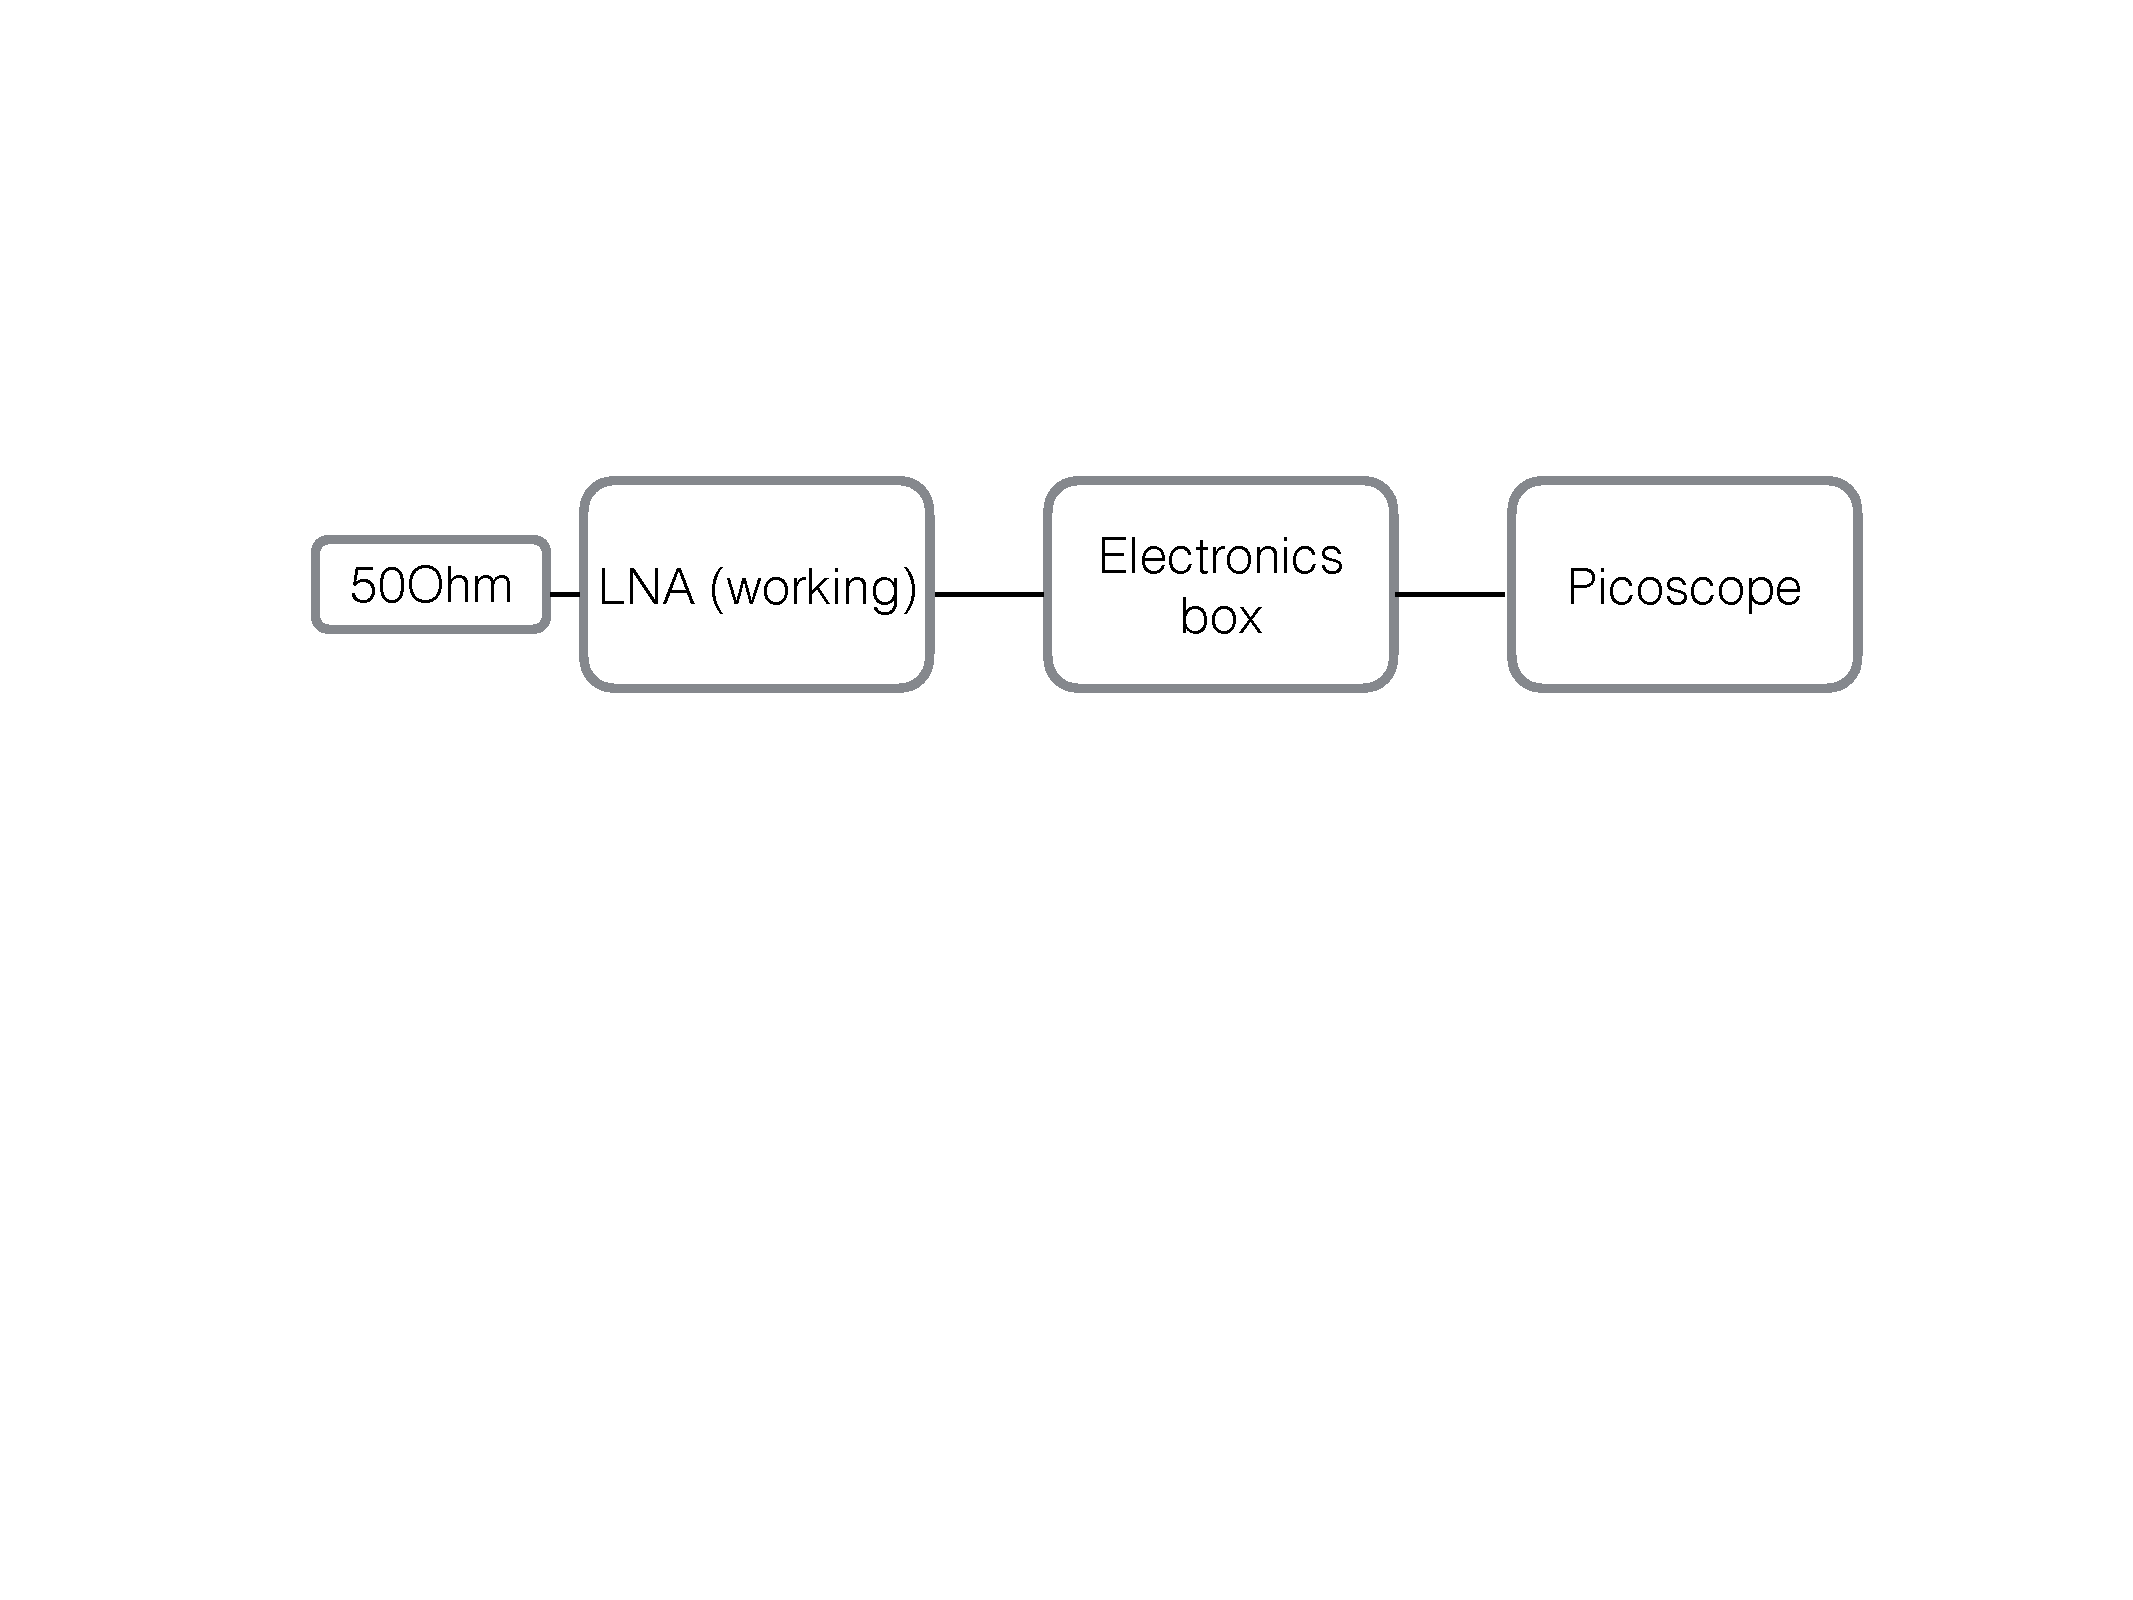
\includegraphics[width=0.60\linewidth]{setupbox.pdf}}
  \caption{setup to evaluate  the electronics box characteristics. The
    LNA and the  load are installed in a LNA box  with an antenna over
    it, but the antenna is NOT connected.}
  \label{fig:setupbox}
\end{figure}
This setup allows us to compare all the boxes with the same reference,
i.e. 300K of  the 50Ohm load. We acquire data  (10 waveforms) with the
Picosope  (4MS/s,  2ms/div)  for  each  box.  The  mean  and  standard
deviation  are  reported  in the  table~\ref{tab:boxtab}.   (reminder:
after the box 100mV=1dB)
\begin{table}[h!]
  \centering
  \caption{average and RMS measurement of the electronics boxes}
  \label{tab:boxtab}
  \begin{tabular}{|c||c|c|c|c|c|c|c|c|c|}
    \hline
    box number & 11  & 10 & 09 & 08 & 05 & 04 & 03 & 02 & 06 \\
    \hline
    station & Gilda  & Santy &  Jorge & Nono & Gringa & - & Eva & Rula & -  \\
    \hline
    average (baseline)[mV] & -469 & -291 &  -270 & -477 & -305 & -548 & -450 & -445 & -774 \\
    \hline
    standard dev  [mV] & 47 & 97 & 40 & 86 & 52 & 83 & 58 & 43 & 50 \\
    \hline
  \end{tabular}
\end{table}
\\
\textbf{notes at data taking}
\begin{itemize}
\item box 09: baseline varies with time ($\simeq$ 1mV/min)
\item box 08: remeasured at $ average = -438 mV$ and $\sigma = 60 mV$
\item box 04: has peaks every 10ms
\item box 03: baseline varies with time ($\simeq$ 1.5mV/min)
\item box 02: baseline varies with time (from -430 to -443 in the first minute, -445 after two minutes)
\item box 06: has peaks every 10ms
\end{itemize}

\paragraph{remarks}
\begin{enumerate}
\item  One can see  that the  baselines are  quite different,  this of
  course   depends   on   how   much  was   rotated   the   adjustable
  resistor. However when  we look at the installation  sheet, for four
  detectors (Gilda, Santy, Eva, and Rula) the baseline was not changed
  at the installation, that means  we can directly compare the average
  values  in the table~\ref{tab:boxtab}.   We see  that Eva,  Rula and
  Gilda differ  by less  than 0.2dB, but  Santy's baseline  differs by
  around 150 mV (1.5dB).
\item A second  remark is about the RMS, one  can see two populations:
  one around 50mV and one around 90mV. This is strange because the RMS
  should not depend on the  adjustable resistor settings, it should be
  approximately the  same for all the  boxes because the  input is the
  same. This problem has to  be investigated because the RMS should be
  a direct measurement of the input noise, so a difference of a factor
  2 is worrying.
\item  Two boxes  (number 4  and number  6) showed  peaks with  a 10ms
  period  (cf fig~\ref{fig:peaks}).   We still  don't know  where this
  noise comes from.  We sometimes  saw it and then it disappeared, its
  amplitude was also changed by the orientation of the box (containing
  the  LNA  and the  50Ohm  load). It  could  be  an anthropic  signal
  captured  by the  antenna  or some  part  of the  box (the  assembly
  building is very noisy at these frequencies).
  \begin{figure}[!ht]
    \centering
    \hspace*{-3ex}
    \subfigure{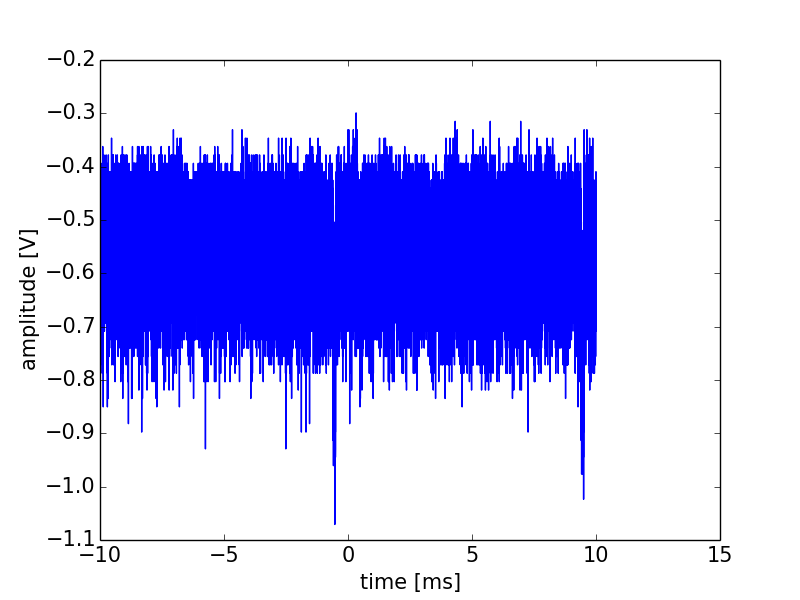
\includegraphics[width=0.49\linewidth]{peaks.png}}
    \subfigure{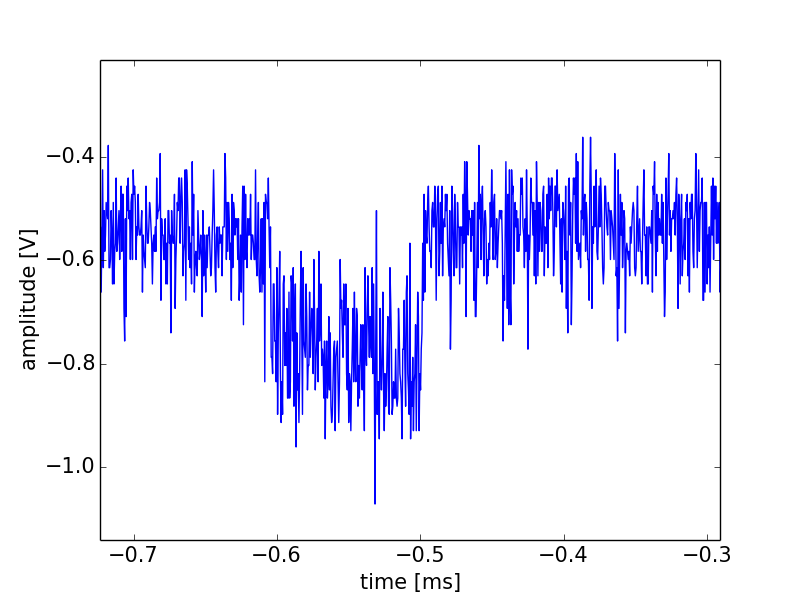
\includegraphics[width=0.49\linewidth]{peaks2.png}}
    \caption{example of trace of the box 4 (left) and zoomed (right)}
    \label{fig:peaks}
  \end{figure}
\item As for the time varying baseline, this could be explained by the
  warm up time  of the electronics.  Mari did  a longer measurement of
  box9.  The results are  plotted in the fig~\ref{fig:box9vstime}, the
  baseline drops by a few tens of mV in 30 minutes.  The decrease rate
  gets smaller with time (the derivative gets close to zero).
  \begin{figure}[!ht]
    \centering
    \hspace*{-3ex}
    \subfigure{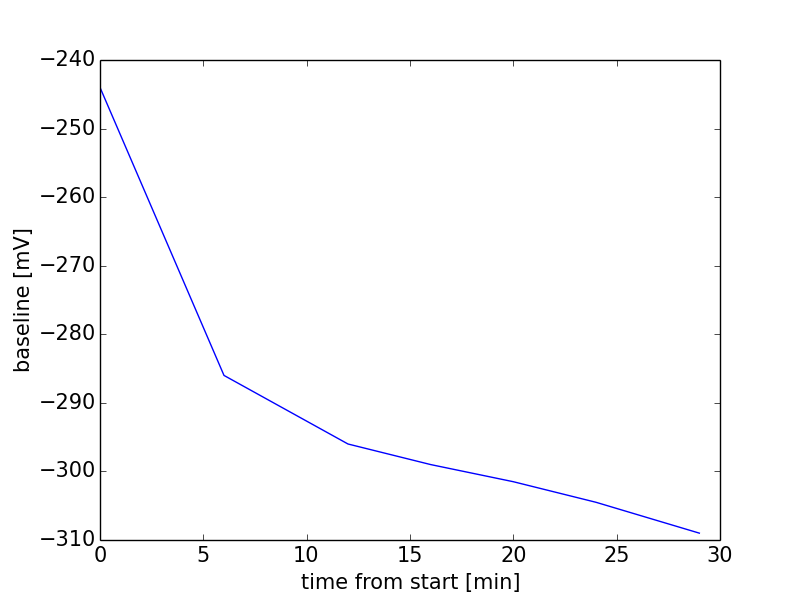
\includegraphics[width=0.49\linewidth]{box9vstime.png}}
    \caption{baseline versus time for the box number 9}
    \label{fig:box9vstime}
  \end{figure}
\end{enumerate}
